% vim:set spell tw=79:

\documentclass[article]{uibk}
\title{Exploitation Techniques and Mitigations}
\author{Alex Hirsch \and Patrick Ober}
\date{2016-01-31}

\usepackage{wrapfig}
\newminted{nasm}{
    fontsize=\scriptsize,
    frame=leftline,
    framesep=2mm,
    autogobble,
    linenos}
\newmintedfile{nasm}{
    fontsize=\scriptsize,
    frame=leftline,
    framesep=2mm,
    autogobble,
    linenos}

\begin{document}

% \maketitle
%
% \section*{Abstract}
% \label{sec:abstract}
%
% \setcounter{tocdepth}{1}
% \tableofcontents
%
% \newpage

\section*{Acknowledgement}

A university course at Rensselaer Polytechnic
Institut\footnote{\url{http://rpi.edu/}} held in Spring 2015 focused on
\textit{Modern Binary Exploitation}. They made their course material available
on GitHub \cite{RPISEC} under the Creative Commons Attribution-NonCommercial
4.0 International
license\footnote{\url{https://creativecommons.org/licenses/by-nc/4.0/legalcode}}.
We reused a lot of their material in this project.

We highly recommend checking them out and having a look at their material for
further details apart from the given references.

\section{Introduction}

Exploiting binaries was comparatively easy ten to fifteen years ago. There were
no special mitigation mechanisms in place denying even the most simplest
exploits. This is the point in time where we will start off. First we talk
about two very simple exploits, namely the Format String Exploit and the Buffer
Overflow in combination with Shell Code. Although there is a huge collection of
exploitation techniques known to the public, we will only look at a very small
fraction of them in this project.

The next section will communicate necessary background knowledge required to
fully grasp the two presented exploits. A short overview about the target
architecture x86 will be given.

After that, both techniques are introduced, followed by the first mitigation
technique, Data Execution Prevention (DEP). From there on we will keep on using
the buffer overflow technique with some adaptations to circumvent DEP. At that
point Return Oriented Programming (ROP) is introduced, directly leads to
Address Space Layout Randomization (ASLR) the follow-up mitigation mechanism.
Again the buffer overflow technique can be adapted to break ASLR through the
use of additional information.

Since neither DEP nor ASLR provide significant protection against even this
simple technique, an additional mitigation has been put into place in the form
of Stack Cookies.

An outlook will be given after bypassing Stack Cookies by looking at Control
Flow Integrity (CFI).

Examples will be provided along the way support the reader and provide some
additional explanation. Finally we will conclude with a word about other
architectures (x86\_64 and ARM) followed by a recap about this project.

\subsection{Main Assumption}

Throughout this work we assume that we know the target binary (and the
libraries it uses). Let us show that this assumption is quite reasonable to
make by looking through the eyes of the adversary. An attacker who wants to
penetrate a target machine would most likely choose the easiest path, by
exploiting the weakest link. Most machines relevant to an attacker's interest
will provide multiple services. Consider following scenario:

The main server of a small business company runs a homemade communication
service for interaction between them and their clients. The attacker has no
access to the source or binary of this communication service's daemon running
on the target machine. But along with it a commonly used web server is
listening on port 80. Getting the source (and binary) of the web server is much
easier therefore an attacker would pick this entry point over the communication
service daemon.

\begin{listing}[h!]
    \begin{code*}{linenos=false}
        <!DOCTYPE HTML PUBLIC "-//IETF//DTD HTML 2.0//EN">
        <html><head>
        <title>400 Bad Request</title>
        </head><body>
        <h1>Bad Request</h1>
        <p>Your browser sent a request that this server could not understand.<br />
        </p>
        <hr>
        <address>Apache/2.2.22 (Ubuntu) Server at ovinnik.canonical.com Port 80</address>
        </body></html>
        Connection closed by foreign host.
    \end{code*}
    \caption{A web server's response to a misspelled request}
    \label{src:http_response}
\end{listing}

\Cref{src:http_response} shows a possible response of a web server when
receiving an invalid request. The web server tells us his exact version and
since it also provides information about the operating system (distribution) an
attacker can easily mimic this setup to test and tweak his exploits. Exploits
may already be known to the public if the used version is not up-to-date. An
attacker could easily reuse them.

\section{Platform x86}

This section will teach necessary background knowledge about the target
platform to fully conceive the following techniques. But first let us elaborate
why x86 has been chosen.

At the time these techniques (and their related mitigations) were established,
x86 was the most common platform. The majority of related material found on the
internet covers x86, and many exploitation techniques can be translated from
x86 to other architectures with ease.

A more detailed overview can be found on
Wikipedia\footnote{\url{https://en.wikipedia.org/wiki/X86}} and if this is not
enough for you, consider the Intel
Manual\footnote{\url{https://www-ssl.intel.com/content/www/us/en/processors/architectures-software-developer-manuals.html}}
for a more profound insight.

\subsection{CPU and registers}

\begin{figure}[htpb]
    \centering
    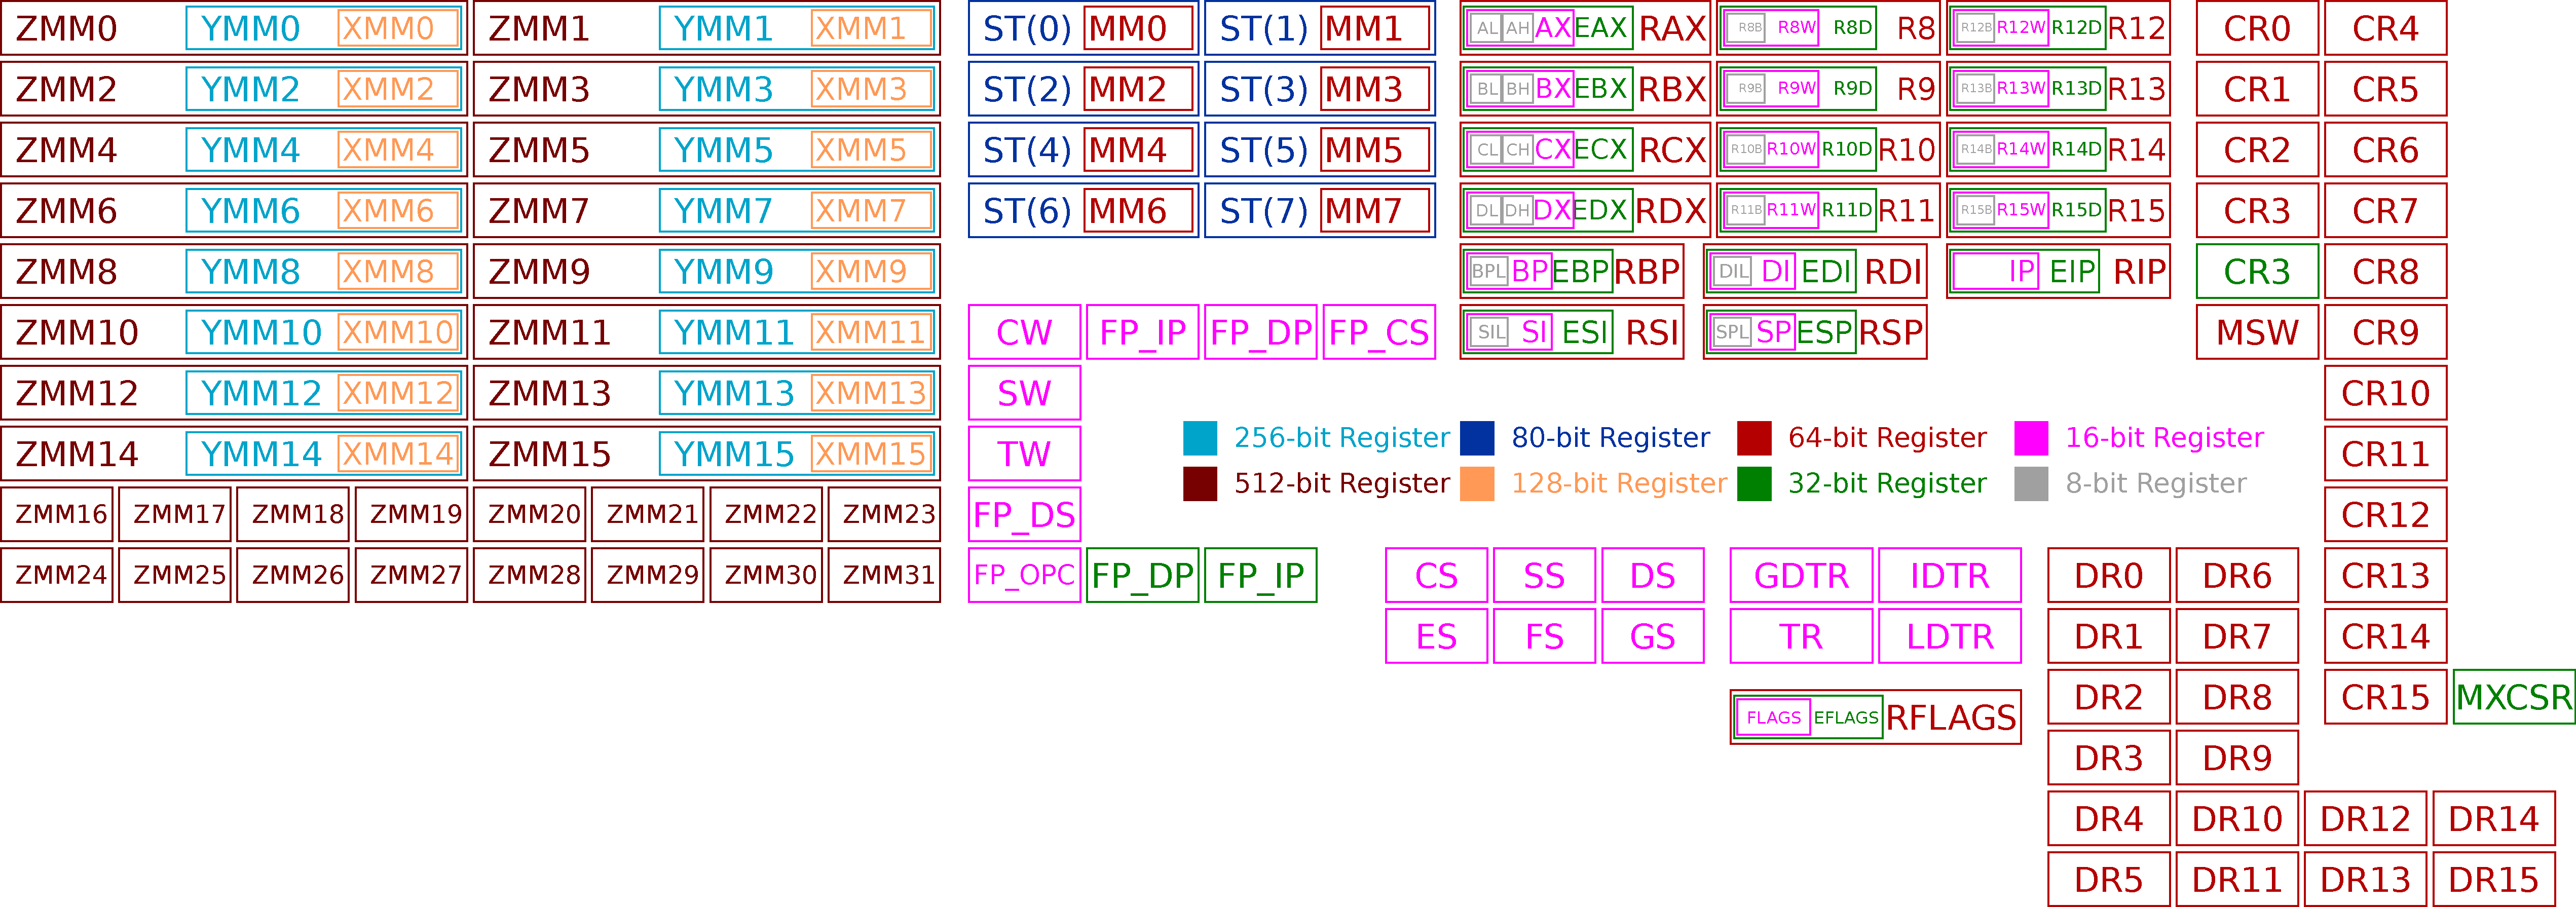
\includegraphics[width=\textwidth]{gfx/x86_registers.pdf}
    \caption{Register overview including \SI{64}{\bit} extension}
    \label{fig:registers}
\end{figure}

\Cref{fig:registers} (from
Wikipedia\footnote{\url{https://en.wikipedia.org/w/index.php?title=X86&oldid=696308590\#/media/File:Table_of_x86_Registers_svg.svg}})
shows an overview of registers available on the x86 platform. While there are
dedicated registers for floating pointer operations and registers with hardware
protection (segment registers) we will only focus on nine commonly used
registers.

\begin{minipage}[t]{0.4\textwidth}
    \begin{description}
        \item[\texttt{EAX}] Accumulator Register
        \item[\texttt{EBX}] Base Register
        \item[\texttt{ECX}] Counter Register
        \item[\texttt{EDX}] Data Register
        \item[\texttt{ESI}] Source Index
        \item[\texttt{EDI}] Destination Index
        \item[\texttt{EBP}] Base Pointer
        \item[\texttt{ESP}] Stack Pointer
        \item[\texttt{EIP}] Instruction Pointer
    \end{description}
\end{minipage}
\begin{minipage}[t]{0.6\textwidth}
    \begin{figure}[H]
        \centering
        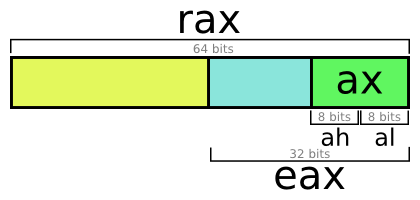
\includegraphics[width=0.8\textwidth]{gfx/single_register.png}
        \caption{Addressing specific parts of a register including \SI{64}{\bit} extension}
        \label{fig:single_register}
    \end{figure}
\end{minipage}
\bigskip

The instruction pointer \texttt{EIP} points to the next instruction in memory
which will be executed the subsequent cycle. Stack pointer \texttt{ESP} and
base pointer \texttt{EBP} are used for stack management which is vital to call
and return from multiple functions properly. The remaining six registers are
used for arithmetic and memory operations as well as passing arguments
(parameters) for system calls. Their values can either be interpreted as
integers or pointers.

Note that these registers can be addressed partially allowing one to write only
to the lower \SI{16}{bit}, for example, as displayed in
\cref{fig:single_register} taken from \textit{null
programm}\footnote{\url{http://nullprogram.com/img/x86/register.png} on
December 2015}.

The CPU comes with protection mechanisms which allows the operating system
kernel to limit other processes' privileges. This mechanism is known as
\textit{protection rings} (Ring 0 -- Ring 3). The kernel runs \emph{in} Ring 0
(most privileged) and switches to Ring 3 (least privileged) when a normal
process is scheduled. A system call is invoked by the process if it needs
something beyond its scope. The kernel takes over, deals with the request and
returns execution back to the process. This is known as \textit{context switch}
and switching between Rings happens along with it.

\subsection{System Calls}

As already mentioned in the previous paragraph, a process only has limited
capabilities and the kernel has to take over to fulfill certain (more
privileged) operations. The operating system's documentation tells you which
system calls are available (on which platform) and what parameters
each of them requires. Let us illustrate this with an example: On x86 Linux the
system call
number 4 (starting from 0) is the \texttt{sys\_write} system call which writes
data to a file descriptor. It takes three arguments, the file descriptor to
write to, a pointer to the start of the data which should be written and the
length of the data. The number of the system call together with these three
parameters are placed in the \texttt{EAX}, \texttt{EBX}, \texttt{ECX},
\texttt{EDX} respectively. To invoke the system call issue following
instruction:

\begin{nasmcode*}{linenos=false}
    int     0x80
\end{nasmcode*}

Nowadays you may encounter a different mechanism for system calls using Virtual
Dynamic Shared Objects (vDSO). This goes beyond our scope here, we will use the
previously mentioned mechanism in our exploits as they work side by side.
Consult the corresponding man
page\footnote{\url{http://man7.org/linux/man-pages/man7/vdso.7.html}} for
further reading.

\subsection{Memory}

Physical memory is managed by the operation system kernel by utilising the
Memory Management Unit (MMU). Each process' address space is virtualized and
memory operations are translated on-the-fly by the MMU. Physical memory is
segmented into \textit{pages} (typically \SI{4}{\kibi\byte} in size) and each
page can be mapped \emph{into} the virtual address space of one or more
(shared) processes.~\cite[pp.~400]{unix_interals}

The main parts located inside the (virtual) address space of a process are the
executable itself with its \texttt{.text} and \texttt{.data} section, the heap
(used for dynamic data), the stack (used for local variables and function
calling) and libraries.

\subsection{Endianness}
\label{sub:endianness}

\begin{figure}[H]
    \centering
    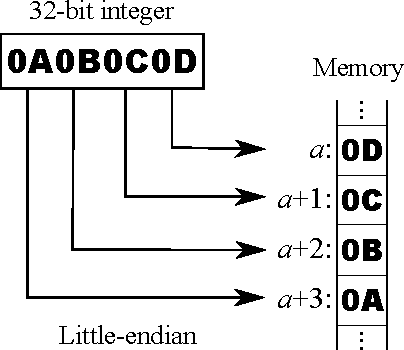
\includegraphics[width=0.35\textwidth]{gfx/little_endian.pdf}
    \caption{Placement of bytes in memory in little-endian}
    \label{fig:little_endian}
\end{figure}

Endianness refers to the byte order used when storing data in memory (or
transmitting it over the network). x86 uses little-endian which is described in
\cref{fig:little_endian} (from
Wikipedia\footnote{\url{https://en.wikipedia.org/w/index.php?title=Endianness&oldid=696417697\#/media/File:Little-Endian.svg}}).
The least significant byte of a word is placed at the lower memory address and
successive bytes are placed as the memory address increases. We will later
refer back to this when needed. The related Wikipedia
page\footnote{\url{https://en.wikipedia.org/wiki/Endianness}} goes into more
detail about this than we need.

\subsection{Calling Convention}
\label{sub:calling_convention}

A calling convention defines how function calls should be implemented. What
calling convention is used depends on the platform, toolchain and compiler
settings. Let us exhibit what the convention defines and what convention we are
using (cdecl).

\begin{minipage}[t]{0.48\textwidth}
    Convention defines:
    \begin{itemize}
        \item Where to place arguments
        \item Where to place return value
        \item Where to place return address
        \item Who prepares the stack
        \item Who saves which register
        \item Who cleans up\\
            (caller or callee)
    \end{itemize}
\end{minipage}\hfill
\begin{minipage}[t]{0.48\textwidth}
    C Declaration (cdecl):
    \begin{itemize}
        \item Arguments on stack (reverse order)\\
            stack aligned to \SI{16}{\byte} boundary
        \item Return via register (\texttt{EAX} / \texttt{ST0})
        \item \texttt{EAX}, \texttt{ECX}, \texttt{EDX} saved by the caller\\
            rest saved by the callee
        \item On stack:\\
            old instruction pointer (\texttt{IP})\\
            old base pointer (\texttt{BP})
        \item Caller does the cleanup
    \end{itemize}
\end{minipage}

\section{Format String Exploits}

The first exploitation technique we will discuss builds upon the interpretation
of format strings. \texttt{printf} is a C function of the standard library
which will interpret such strings and print them to \texttt{stdout}. As the
name already tells you, the supplied string contains \textit{formatter}
describing how to handle additional arguments. If you are unfamiliar with
\texttt{printf} please have a look at the man
page\footnote{\url{http://linux.die.net/man/3/printf}} now.

Taking a closer look at \texttt{printf} we can see that its first argument is a
format string followed by a variable number of additional arguments.
\texttt{stdarg.h} describes a common implementation of this together with a
small example in their man
page\footnote{\url{http://linux.die.net/man/3/stdarg}}. As in that example,
\texttt{printf} trusts you that the number of arguments supplied is equal (or
greater) than the number of formatters. Calling \texttt{printf} with the format
string \texttt{"\%d + \%d = \%d"}, for instance, assumes that (at least) three
additional arguments are given.

\begin{listing}[h!]
    \begin{minipage}[t]{0.4\textwidth}
        \cfile{../src/format_string/format.c}
    \end{minipage}\hfill
    \begin{minipage}[t]{0.5\textwidth}
        \begin{code*}{linenos=false}
            > gcc -o format format.c


            > echo foobar | ./main
            You entered:
            foobar


            > echo AAAABBBB | ./main
            correct


            > echo '%08x' | ./main
            You entered:
            bfd98ed4
        \end{code*}
    \end{minipage}
    \caption{Program vulnerable to Format String Exploits}
    \label{src:format_string_exploit}
\end{listing}

The exploit comes from the notion that a format string provided by an attacker
gets interpreted. The program shown in \cref{src:format_string_exploit} will
take an arbitrary string from \texttt{stdin} and pass it on to \texttt{printf}.
For simple inputs (not containing formatter) this works fine. But as soon as
formatter are provided, \texttt{printf} accesses the locations where the
corresponding arguments \emph{would} be located. From the calling convention
described in \cref{sub:calling_convention} we know that these arguments
\emph{would} be located on the stack, therefore \texttt{printf} will print
whatever lies on the stack at these positions instead.

An attacker in this scenario wants to get a hold of the hardcoded password
stored in \texttt{passwd}. Since local variables are placed on the stack
\texttt{printf} will be able to read the password if enough formatters are
provided:

\begin{code*}{linenos=false}
    > python -c 'print "%08x." * 10' | ./main
    bf920c14.00000064.b77de29e.00000000.00000000.b77fedf8.bf920d94.00000000.41414141.42424242.
\end{code*}

Here we use Python to craft the format string containing ten identifiers for
us. As we can see the password is printed (ASCII encoded). Byte order is
swapped because of endianness (see \cref{sub:endianness}). Apart from the
password we also gather a bunch of pointers, these can be used later on to
break ASLR (see \cref{sub:info_leak}).

We would like to point the reader to the book \textit{Hacking: The Art of
Exploitation}~\cite[pp.~167]{art_of_exploitation} for more details about this
and following techniques. We will come back to this technique later on to show
that \texttt{printf} enables even more sophisticated attacks.

\section{Buffer Overflow}

The second type of exploits we'll look at is known as Buffer Overflows and as
on may already derive from the name, this is about submitting more data to a
buffer than it was originally designed for. This setup can be exploited when
bound checking is done wrong or not at all. An attacker is therefore able to
overwrite memory behind the buffer's location.

\subsection{Disabling Mitigations}

The three mitigation mechanisms DEP, ASLR and Stack Cookies are enabled by
default nowadays and as mentioned in the introduction we start off at a pointer
where these mechanisms were not. So to run the provided examples we first have
to disable them. DEP and Stack Cookies can be disabled via compiler flags to
the extend necessary using \texttt{-z execstack} and
\texttt{-fno-stack-protector} respectively.

ASLR can be disabled globally so that \emph{new} process' has an unscrambled
memory layout:

\begin{code*}{linenos=false}
    > echo 0 > /proc/sys/kernel/randomize_va_space
\end{code*}

Writing \texttt{2} instead of \texttt{0} will switch ASLR back to its default
state. Root privileges are, of course, required for this. There is also another
way by invoking \texttt{setarch}:

\begin{code*}{linenos=false}
    > setarch `arch` -R ./binary
\end{code*}

\subsection{The Exploit}

The consequences of an exploited buffer overflow depend on where the buffer is
located. The most interesting location would of course be the stack because,
apart from local variables and arguments, it holds the return address of a
function. But buffers located inside the heap or static may also be viable
options. Common terms related to these scenarios are \textit{stack smashing}
and \textit{heap corruption}. We will talk about heap corruption later on when
breaking ASLR, for now we focus our attention on stack smashing.

\begin{figure}[H]
    \centering
    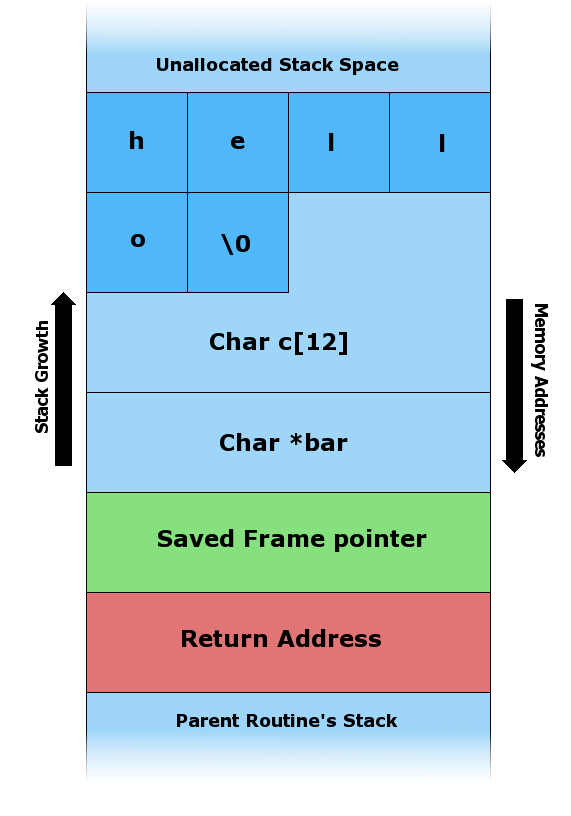
\includegraphics[width=0.4\textwidth]{gfx/stack_smash.png}
    \caption{Stack frame containing a buffer}
    \label{fig:stack_frame}
\end{figure}

Lets start off by examining the stack containing a buffer \texttt{c} as local
variable, see \cref{fig:stack_frame}. Right now the buffer holds the string
\texttt{"hello"} followed by a terminator. Since it has been allocated
to hold a maximum of \SI{12}{\byte} this fits. If data is written to the buffer
larger than \SI{12}{\byte} the following variable (or parameter) \texttt{bar}
will be overwritten, followed by the saved frame pointer and the return
address. If even more data is supplied the following stack frame will be
overwritten in the same manner.

If an attacker can provide the data written to the buffer and no (or wrong)
bound checking is done, he is able to inject arbitrary (malicious) code into
the stack frame. This could be, for instance, be used to overwrite a flag
indication whether an authentication has been performed successfully or not.
But since this is pretty forward lets go beyond that and see what happens when
changing the return address.

\begin{listing}[h!]
    \begin{minipage}[t]{0.37\textwidth}
        \cfile{../src/buffer_overflow/overflow.c}
    \end{minipage}\hfill
    \begin{minipage}[t]{0.63\textwidth}
        \codefile{../src/buffer_overflow/overflow_objdump.txt}
    \end{minipage}
    \caption{Program vulnerable to buffer overflows}
    \label{src:buffer_overflow}
\end{listing}

As shown in \cref{src:buffer_overflow} we have a buffer suited for
\SI{20}{\byte} but without any bound checking. If the provided input is longer,
we will be able to overwrite the return address. Lets have a look at the
resulting binary utilizing \texttt{objdump}.

Looking at lines 13 and 23 we can infer that the buffer will start
\SI{28}{\byte} (\texttt{0x1c}) before the base pointer. Hence we have to supply
\SI{32}{\byte} (28 + 4) of arbitrary data followed by the address where we want
to jump to. Lets jump into the function \texttt{mordor} located at
\texttt{0x804849b}, keep in mind that the byte order needs to be swapped.

\begin{code*}{linenos=false}
> python -c "print 'A'*32 + '\x9b\x84\x04\x08'" | setarch `arch` -R ./overflow
Enter text:
You entered: AAAAAAAAAAAAAAAAAAAAAAAAAAAAAAAA��
One does not simply jump into mordor()!
Segmentation fault (core dumped)
\end{code*}

\texttt{mordor} has been executed successfully. Despite the segmentation
fault one can see that return address has been overwritten successfully.

\section{Shell Code}

While this is neat and can certainly be useful to an adversary, stack smashing
also enables us to inject arbitrary code into a program. Contrary to the
previous section the target machine will execute code provided by the attacker.
This can be achieved by bending the return address into the buffer used for the
exploit. Provided instructions will be executed upon return. Shell code is a
piece of (binary) code which opens up a shell that reads and executes commands
from an attacker. This example is taken from Dhaval Kapil's
blog\footnote{\url{https://dhavalkapil.com/blogs/Shellcode-Injection/} on
December 2015} there is also a section about this in \textit{Hacking: The Art
of Exploitation}~\cite[pp.~281]{art_of_exploitation}.

\subsection{Crafting Shell Code}

\begin{listing}[h!]
    \begin{minipage}[t]{0.4\textwidth}
        \nasmfile{../src/shell_code/shellcode.asm}
    \end{minipage}\hfill
    \begin{minipage}[t]{0.5\textwidth}
        \codefile{../src/shell_code/shellcode_objdump.txt}
    \end{minipage}
    \caption{Assembly code opening up a shell upon execution}
    \label{src:shell_code}
\end{listing}

The piece of assembly shown in \cref{src:shell_code} sets up the parameters for
the \texttt{execve} system call and than invokes it to replace the currently
running process with a shell. \texttt{execve} takes three arguments, a string
of the program to execute (here \texttt{"/bin//sh"} + terminator), a list of
arguments for that program and a list of environment variables. Its system call
number is 11 and it will accept \texttt{NULL} for both lists. The double slash
in the first argument is used to prevent null bytes inside the shell code. The
function which reads the shell code may truncate it upon reading a null byte,
therefore we have to work around this without changing the underlying
semantics.

Running this code through an assembler yields binary code, shown in
\cref{src:shell_code}, which will be part of the payload.

\begin{code*}{linenos=false}
    \x31\xC0\x50\x68\x2F\x2F\x73\x68\x68\x2F\x62\x69\x6E\x89\xE3\x50\x89\xE2\x53\x89\xE1\xB0\x0B\xCD\x80
\end{code*}

\subsection{Examining the Target Binary}

Finding the starting location of our buffer will be a little bit more
complicated, we cannot read it directly from the binary of the target program
so, in \cref{src:shell_code2}, we'll examine it in a debugger .

\begin{listing}[h!]
    \begin{minipage}[t]{0.4\textwidth}
        \cfile{../src/shell_code/vuln.c}
    \end{minipage}\hfill
    \begin{minipage}[t]{0.5\textwidth}
        \codefile{../src/shell_code/vuln_gdb.txt}
    \end{minipage}
    \caption{Examining the target binary in \texttt{gdb}}
    \label{src:shell_code2}
\end{listing}

Now we know that the buffer will be located at \texttt{0xbffff4bc} (saved base
pointer will be at \texttt{0xbffff528}) at runtime, but it may be offset a few
bytes when run without debugger. This happens because environment variables and
meta information, like the program name, determine the stack starting position
(stack is placed right before environment variables). Hence we may not hit the
first instruction of our shell code right away, but since the buffer is bigger
than the actual payload we can improve our odds by prefixing the shell code
with \texttt{NOP} instructions. As long as the return address points somewhere
into this sequence of \texttt{NOP}s the CPU will \emph{slide} to the first
instruction of the shell code. Therefore this is known as a
\textit{\texttt{NOP} Sled}. We append some arbitrary data to the shell code as
offset to overwrite the return address. This is also illustrated in
\cref{fig:shell_code} where \textit{target} is new return address supplied by
the attacker. Using the maximum amount of \texttt{NOP}s possible would also be
a viable option, here we just went with the original example.

\begin{figure}[H]
    \centering
    \usetikzlibrary{arrows.meta}
\usetikzlibrary{shapes.multipart}

\tikzstyle{block} = [
	draw,
	align=center,
	rectangle,
]

\tikzstyle{block split} = [
	block,
	rectangle split,
	rectangle split horizontal,
	rectangle split part align=base,
]

\tikzstyle{ptr}=[
	-{Latex[length=2.7mm]}
]

\begin{tikzpicture}

\node[block split] (payload) {
	\nodepart{one}    \texttt{NOP} Sled
	\nodepart{two}    Shell Code
	\nodepart{three}  AAA\dots AAA
	\nodepart{four}   \textit{target}
};

\draw [ptr] (payload.four south) -- +(0,-0.5) -| (payload.one south);

\end{tikzpicture}

    \caption{Putting the payload together}
    \label{fig:shell_code}
\end{figure}

Lets first calculate the distance between the start of the buffer and the
return address. The return address will be located \SI{4}{\byte} after the
saved base pointer location.

\[(\texttt{0xbffff528} + 4) - \texttt{0xbffff4bc} = 112\]

We prefix our shell code with a \texttt{NOP} Sled consisting of \SI{40}{\byte}
(opcode for \texttt{NOP} is \texttt{0x90}). Since our shell code is \SI{25}{\byte}
long we add 47 \texttt{'A'}s to gap the remaining distance. Lastly we have to add
the new return address which should point to the \texttt{NOP} Sled's center.

\[\texttt{0xbffff4bc} + 20 = \texttt{0xbffff4d0}\]

\subsection{Gimme that Shell already}

\codefile[linenos=false]{../src/shell_code/run.txt}

After injecting the payload we get a few lines of garbage and receive a prompt
by hitting return a few times. You can enter commands and receive output like
usual.

\section{Data Execution Prevention (DEP)}

\section{Return Oriented Programming (ROP)}

\section{Address Space Layout Randomization (ASLR)}

\subsection{Info Leak}
\label{sub:info_leak}

\section{Stack Cookies}

\section{Control Flow Integrity (CFI)}

\section{Other Architectures}

\section{Conclusion}

\bibliography{references}

\end{document}
